%!TeX spellcheck = fr-FR
% Nicolas Castel PhD thesis -- (C) 2023

\documentclass[thesis]{subfiles}

\begin{document}

\begin{otherlanguage}{french}

\renewcommand{\thesection}{\arabic{section}}
\renewcommand{\thesubsection}{\arabic{section}.\arabic{subsection}}
\renewcommand{\thefigure}{R\arabic{figure}}
\setcounter{figure}{0}
\titlecontents{section}[4.8em]{\addvspace{0.1em}}{\contentslabel{2.2em}}{}{\titlerule*[1pc]{.}\contentspage}[]

\chapter*{Résumé en français}
\startcontents[chapters]
\printpartialtoc

\section*{Introduction}

\todo{5 à 10 pages}

Les procédés industriels de séparation des gaz sont largement utilisés pour fournir des réactifs purifiés et des gaz inertes aux industries chimiques, sanitaires, agricoles et alimentaires pour les industries de la chimie, de la santé, de l'agriculture et de l'alimentation. Ils peuvent également être utilisés pour atténuer l'impact négatif de certaines activités industrielles sur l'environnement : dans les usines de production de béton ou d'acier, les émissions très problématiques de \ce{CO2} pourraient être piégées ; mais aussi dans les usines de retraitement des combustibles nucléaires, des composés radioactifs volatiles peuvent être séparés des autres gaz. Différentes petites molécules comme le diazote, le dioxygène, le dioxyde de carbone, le dihydrogène, le méthane, le protoxyde d'azote ou les gaz rares sont ainsi séparées, purifiées puis stockées. La séparation xénon/krypton étudiée dans cette thèse est communément utilisée pour extraire ces gaz de l'atmosphère, mais l'industrie du nucléaire constitue une source bien plus abondante de xénon et de krypton.

Les procédés industriels de séparation Xe/Kr sont encore bien souvent basés sur la distillation cryogénique de l'air ambiant, ce qui requiert beaucoup d'énergie, une infrastructure complexe et un contrôle minutieux des risques. On peut par exemple évoquer les récents accidents d'exploitation d'usine de séparation de gaz (1997) qui ont été causés notamment par la réaction d'hydrocarbures de l'environnement avec l'oxygène liquéfié de l'usine. Pour éviter les problèmes de sécurité et de coûts importants, de nombreux chercheurs s'attèlent à développer des méthodes de séparation industrielle basées sur l'adsorption dans des matériaux nanoporeux. Ces matériaux nanoporeux sont constitués de pores à l'échelle nanoscopique qui offrent une large surface aux molécules pour y interagir puis s'adsorber. Des procédés industriels basés sur cette technologie existent déjà, ils utilisent notamment le \emph{pressure swing adsorption} (PSA) qui consiste à remplir les pores d'un mélange de gaz à haute pression, puis de récupérer un gaz ainsi purifié. En effet, les pores du matériau permettent l'adsorption préférentielle d'une molécule par rapport aux autres ce qui permet d'augmenter la teneur en une certaine molécule du mélange de sortie. En répétant ce procédé, on peut ainsi séparer les différentes molécules d'un gaz. Dans le cadre de ma thèse, le xénon étant chimiquement proche du krypton, la purification par ce procédé reste un défi majeur. Certains prototypes industriels ont déjà été imaginés, mais la recherche d'un matériau pour effectuer au mieux cette tâche reste aujourd'hui une question ouverte. 

Pour développer un procédé viable, il faut donc choisir avec soin les matériaux que l'on utilise dans ces dispositifs industriels. La recherche se focalise aujourd'hui sur la conception de matériaux toujours plus sélectifs en se basant sur des intuitions chimiques construites au fil des études. Afin d'éviter les expériences coûteuses pour tester tous les matériaux, les criblages computationnel sont de plus en plus utilisés. Ces criblages ou \emph{screenings} en anglais permettent de passer en revu de grandes quantités de structures afin d'en évaluer leur potentiel performance. Tout l'enjeu est donc de former une bonne synergie entre la conception minutieuse de matériaux et la recherche et évaluation rapide des matériaux via des méthodes informatiques. Du côté du traitement informatique des matériaux, les deux défis majeurs sont la génération de données fiables et divers afin de couvrir le spectre des possibles et le développement de nouveaux outils pour l'évaluation rapidement et avec précision les performances de ces matériaux. 

La quantité de matériaux est potentiellement infinie, rien que pour les \emph{metal--organic frameworks} (MOFs) en anglais, plus de 90\,000 structures ont été synthétisées et 500\,000 ont été construits de manière digitale. Pour pouvoir évaluer tous ces matériaux, différentes stratégies ont été élaborées. Certains utilisent des criblages à plusieurs niveaux qui permettent de réduire au fur et à mesure les matériaux à évaluer avec des méthodes plus coûteuses, d'autres se basent sur des algorithmes d'apprentissage statistiques. Cependant peu d'études se focalisent sur les outils de calcul, en eux-mêmes, qui sont souvent davantage adaptés à des calculs sur des structures uniques plutôt que pour être déployés sur des centaines de milliers de structures. Dans cette thèse, je m'emploie donc à développer des outils pour accélérer les procédés de criblages actuels tout en travaillant sur la précision des évaluations de performance. Outre la sélectivité, d'autres variables revêtent une importance significative : la capacité d'adsorption du matériau, la cinétique et la thermodynamique derrière la régénération du matériau (c'est-à-dire en vider les pores). Pour cette raison, ma thèse étudie également les propriétés de transport du xénon et du krypton dans ces matériaux nanoporeux. 

\section*{\'Etude thermodynamique de la séparation Xe/Kr}

En premier lieu, mes travaux ont porté sur l'analyse poussée des corrélations qu'il pouvait exister entre les différentes grandeurs thermodynamiques décrivant la séparation xénon/krypton. Pour cela, la base de données CoRE MOF 2019 a été considéré
La première étude se concentre sur les grandeurs thermodynamiques définies précédemment pour 9,668 structures d'une base de données CoRE MOF 2019. Ces grandeurs seront comparées entre elles via des corrélations et des comparaisons entre basse et haute pression.

Pendant cette thèse, j'ai remarqué des corrélations entre l'enthalpie et la sélectivité. Sur la figure~\ref{fgr:histo_H_resume}, l'enthalpie d'adsorption du xénon est assez bien corrélée au logarithme de la sélectivité à basse pression suggérant ainsi que l'affinité du xénon avec le matériau peut expliquer la sélectivité. Cette corrélation diminue cependant pour les matériaux moins sélectifs. Les matériaux les plus sélectifs ont en effet des pores dont la taille est très favorable à l'adsorption du xénon comme le suggère d'autres études. Pour des gaz nobles, seules les interactions de Van der Waals jouent un rôle important, c'est pourquoi la taille des pores permettent d'expliquer en grande partie l'affinité comparée entre deux molécules de tailles différentes le xénon et le krypton. Ainsi, dans des matériaux avec de petits pores, les phénomènes sont dominés par les interactions entre les pores et l'adsorbat, c'est-à dire par l'enthalpie. Alors que dans de larges pores, les effets entropiques jouent un rôle plus important.

\begin{figure}[h]
\begin{minipage}[t]{.43\textwidth}
\centering
  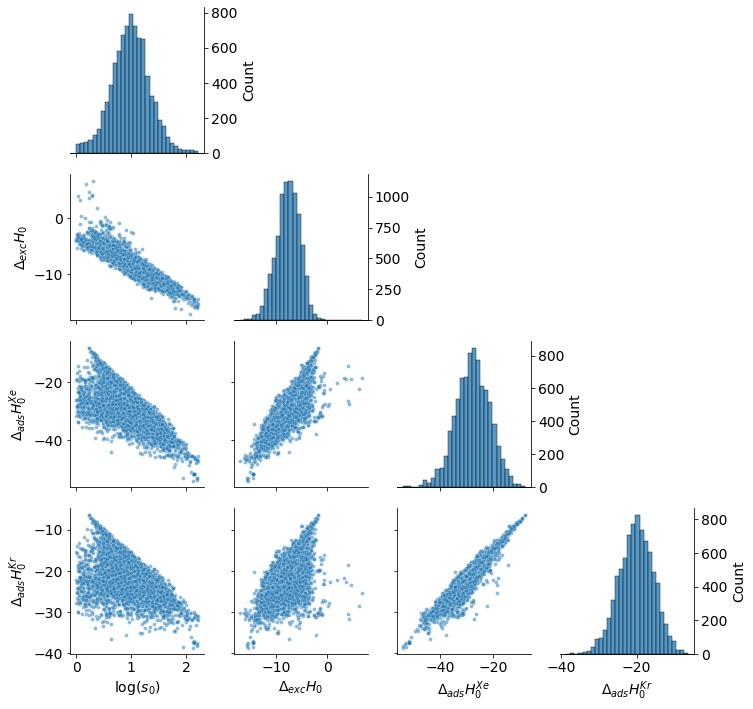
\includegraphics[width=\linewidth]{figures/2-thermo/Enthalpy_0_log.jpg}
  \caption{\small{\ Pour 8401 MOFs avec une sélectivité Xe/Kr favorable ($s\e{0} > 1$), pair-plots entre les différentes grandeurs $\log(s\e{0})$, $\Delta\e{exc}H\e{0}$, $\Delta\e{ads}H\ex{Xe}\e{0}$ et $\Delta\e{ads}H\ex{Kr}\e{0}$ (les enthalpies sont en \si{\kilo\joule\per\mol}) en dehors de la diagonale et la distribution de chaque grandeur sur la diagonale.}}
  \label{fgr:histo_H_resume}
\end{minipage}
\hfill
\begin{minipage}[t]{.5\textwidth}
\centering
  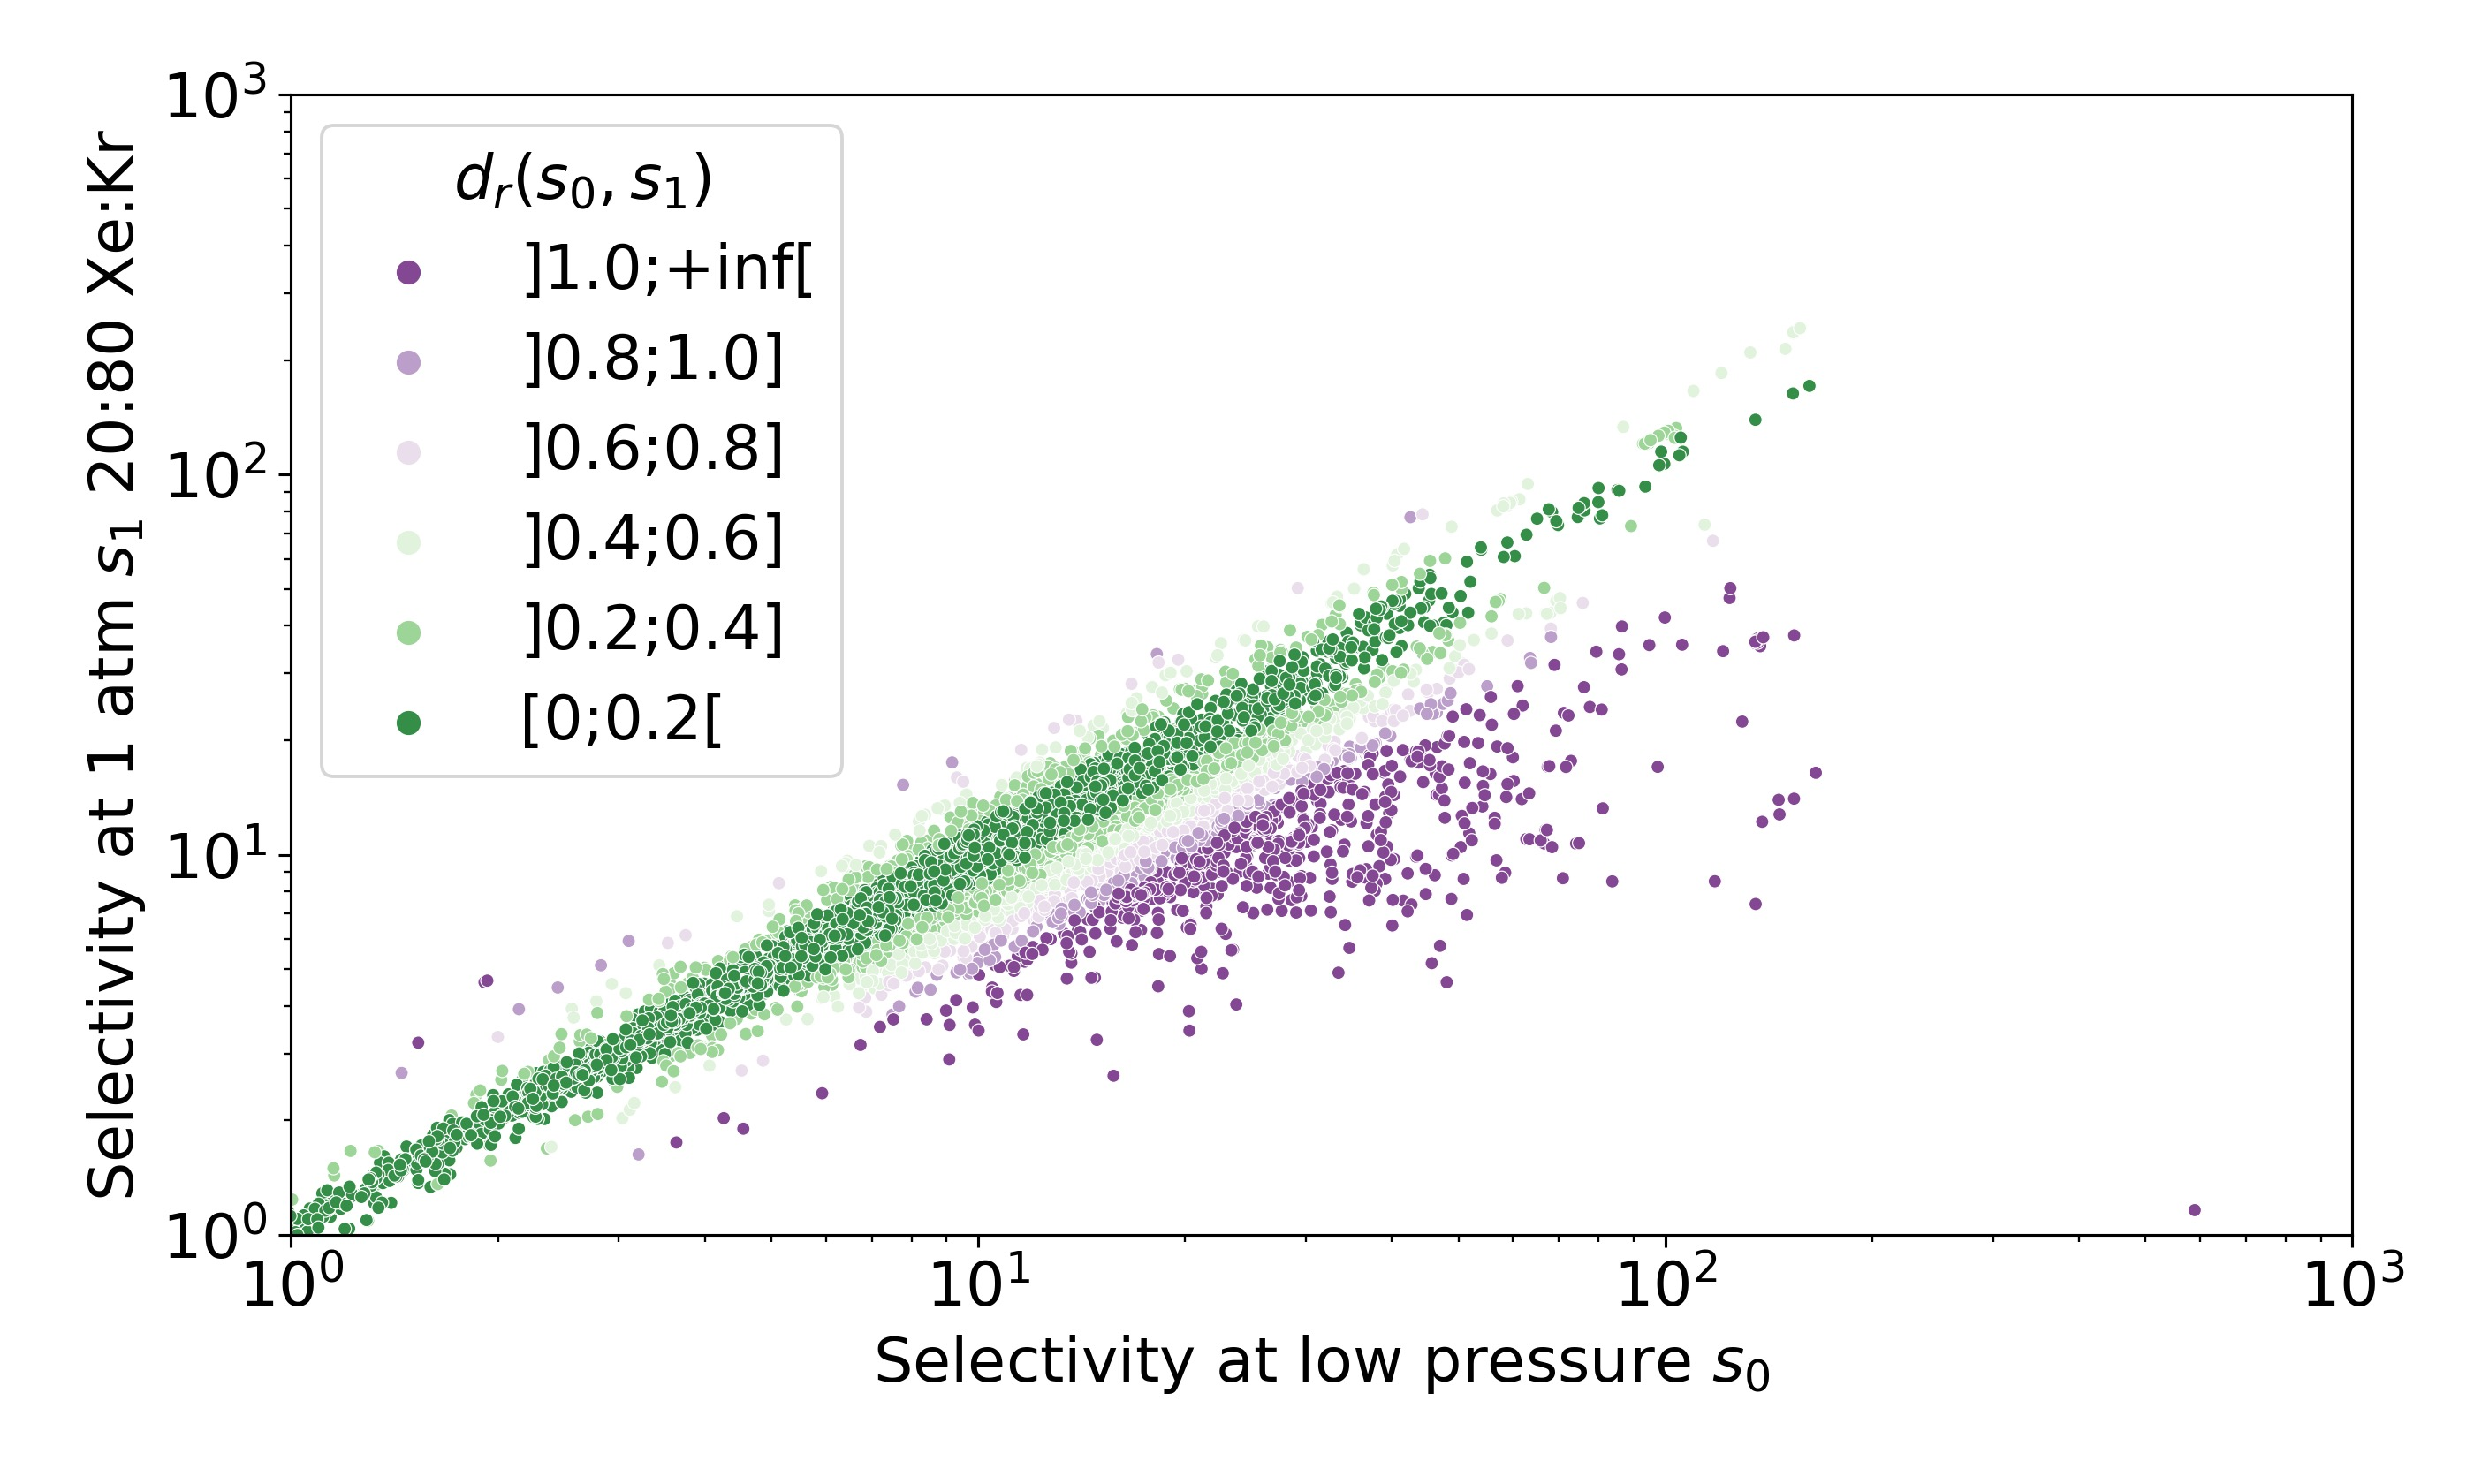
\includegraphics[width=\linewidth]{figures/2-thermo/s_0_vs_s_2080_overview_log.jpg}
  \caption{\small{\ Sélectivité à \SI{1013}{\hecto\pascal} de pression en fonction de la sélectivité à basse pression pour une composition 20\pp{}80 Xe/Kr. Les points sont étiquetés selon la différence relative entre les deux sélectivités. Les points violets ont une grande différence relative entre les sélectivités. }}
  \label{fgr:overview_resume}
\end{minipage}
\end{figure}

D'autre part, nous observons sur la figure~\ref{fgr:histo_H_resume} que l'enthalpie d'échange est très bien corrélée à la sélectivité. Cela peut s'interpréter à l'aide de l'équation suivante $\Delta\e{exc}H= T\Delta\e{exc}S - RT\ln{s}$ dans le cas où $T\Delta\e{exc}S$ est quasi-constante. En effet, l'entropie joue le rôle de bruit d'un point de vue statistique ce qui est confirmé par d'autres figures au chapitre 2 de cette thèse, où l'on observe clairement l'absence totale de corrélation avec la sélectivité. Cette première figure nous renseigne ainsi sur le rôle prédominant de l'enthalpie d'échange pour expliquer la sélectivité observée. 

La figure~\ref{fgr:overview_resume} quant à elle met en évidence la chute de la sélectivité de certains matériaux lorsque l'on passe de la basse pression à la pression ambiante. Cette différence de sélectivité est étudiée à l'aide de l'enthalpie et l'entropie d'échange. Et nous remarquons à nouveau que ce changement de sélectivité est en grande partie expliquée par une augmentation de l'enthalpie d'échange pour ces structures. L'entropie joue encore un rôle relativement mineur sur ce phénomène. L'étude des données thermodynamiques sur un ensemble de 9668 structures nous suggère que l'enthalpie d'échange définie précédemment permet d'expliquer en grande partie les tendances des sélectivités thermodynamiques à haute et basse pression. La séparation xénon/krypton est donc dominée par des effets enthalpiques. 

En étudiant de plus près des matériaux qui perdent de la sélectivité à plus haute pression, ma thèse s'est intéressé de près aux origines microscopiques du changement de sélectivité observé sur la figure~\ref{fgr:overview_resume}. Pour cela, nous allons présenter dans ce résumé une structure problématique en particulier pour illustrer les caractéristiques de la structure. 

Dans d'autres cas, il n'y a pas qu'un seul type de site d'adsorption ni un seul canal unidirectionnel. Le matériau WOJJOV (figure~\ref{WOJJOV_resume}) est un exemple de structure contenant deux types de pores comme on peut le voir sur la représentation graphique et ce qui est confirmé par la validité d'un modèle à 2 sites pour décrire les isothermes corps pur. Le premier type de type est plus petit et a une taille parfaite pour adsorber le xénon. Cela explique pourquoi à basse pression la sélectivité est très bonne $s_0=146$. Lorsqu'on augmente la pression, les sites plus larges commencent à être occupés. Or ces sites plus larges sont moins sélectifs du fait de leur taille. C'est pourquoi la sélectivité diminue grandement et passe à $s_1=14$ à pression ambiante. D'autres structures ayant un système plus complexe de canaux baissent également en sélectivité avec la pression.

\begin{figure*}[h]
\centering
  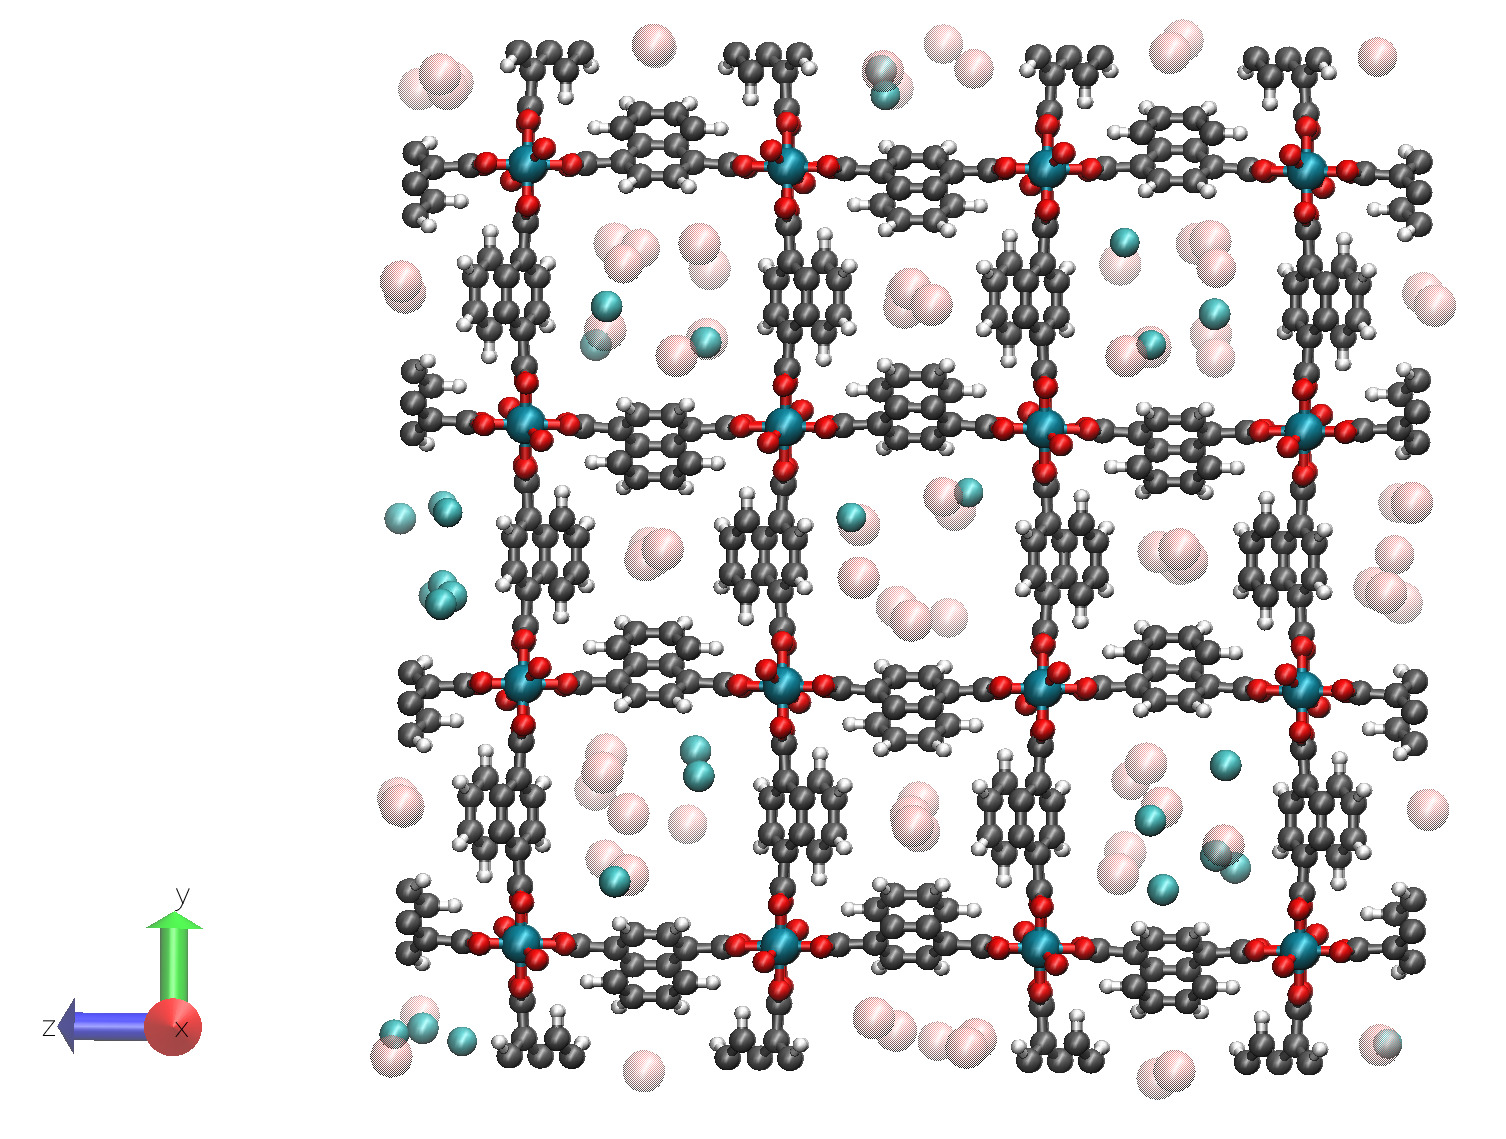
\includegraphics[width=0.4\textwidth]{figures/2-thermo/WOJJOV_clean.jpg}
  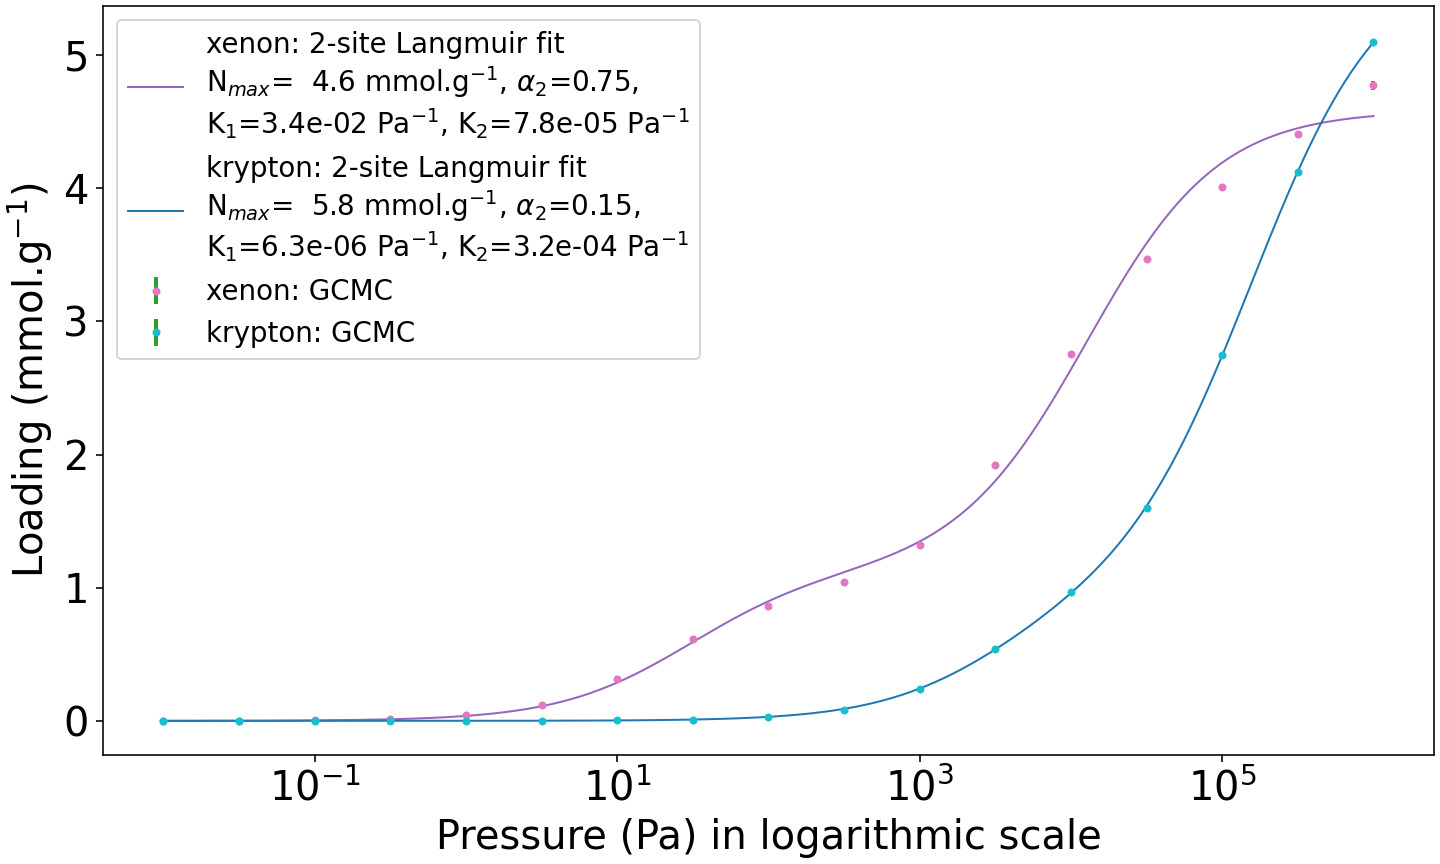
\includegraphics[width=0.4\textwidth]{figures/2-thermo/WOJJOV_clean_isotherm_xenon_krypton_298K.jpg}
  \caption{\small{\ WOJJOV : Représentation d'un MOF [Al(OH)(1,4-NDC)]$\cdot$2(H$_2$O) où NDC signifie naphthalenedicarboxylate. Code couleur : Cu en cyan foncé, C en gris, O en rouge, H en blanc ; Xe en rose and Kr en cyan clair. Sur la droite, les isothermes du xénon et krypton pures à \SI{298}{\kelvin} ainsi qu'un modèle d'isotherme à deux sites.}}
  \label{WOJJOV_resume}
\end{figure*}

La présence de différents types de site et les réorganisations dues aux interactions du mélange Xe/Kr dans la phase d'adsorption permettent d'expliquer à l'échelle moléculaire la différence de sélectivité à basse et haute pression pour un certain nombre d'exemples.

\section*{Développement d'outils de screening}

Comme nous l'avons vu dans la partie précédente, l'enthalpie d'adsorption joue un rôle primordial dans l'explication des performances d'un matériau. Cette enthalpie à basse pression peut être théoriquement calculée grâce à un échantillonnage des énergies d'interaction pour tous les points accessibles de l'espace, mais cette méthode est coûteuse en temps de calcul. C'est pourquoi, les méthodes d'échantillonnage aléatoire des points de l'espace se basant sur les algorithmes Monte Carlo sont plus souvent utilisées (insertion de Widom). Cependant, cet échantillonnage aléatoire ne tient donc pas en compte des informations que l'on a sur les matériaux nanoporeux. En effet, les adsorbats ne se situent pas à des endroits aléatoires et imprévisibles, ils sont souvent au niveau des centres des pores (si la taille est adaptée) ou sur la surface des pores. Nous nous sommes donc intéressés à la possibilité d'exploiter ces informations afin de diminuer le temps de calcul nécessaire à la détermination de l'enthalpie d'adsorption.

La première méthode approchée d'échantillonnage consiste à calculer les énergies sur les n\oe{}uds de Voronoï. Les n\oe{}uds de Voronoï sont des points équidistants à au moins quatre atomes de la structure. Si on considère uniquement les points de Voronoï accessibles, ces points seront situés au centre des pores. La deuxième méthode quant à elle échantillonne les surfaces des pores. Pour cela l'algorithme parcourt les points à la surface des atomes de la structure et y calcule l'énergie d'interaction avec le matériau. 

La deuxième méthode se base sur l

GrAED

\begin{figure}[ht]
    \centering
      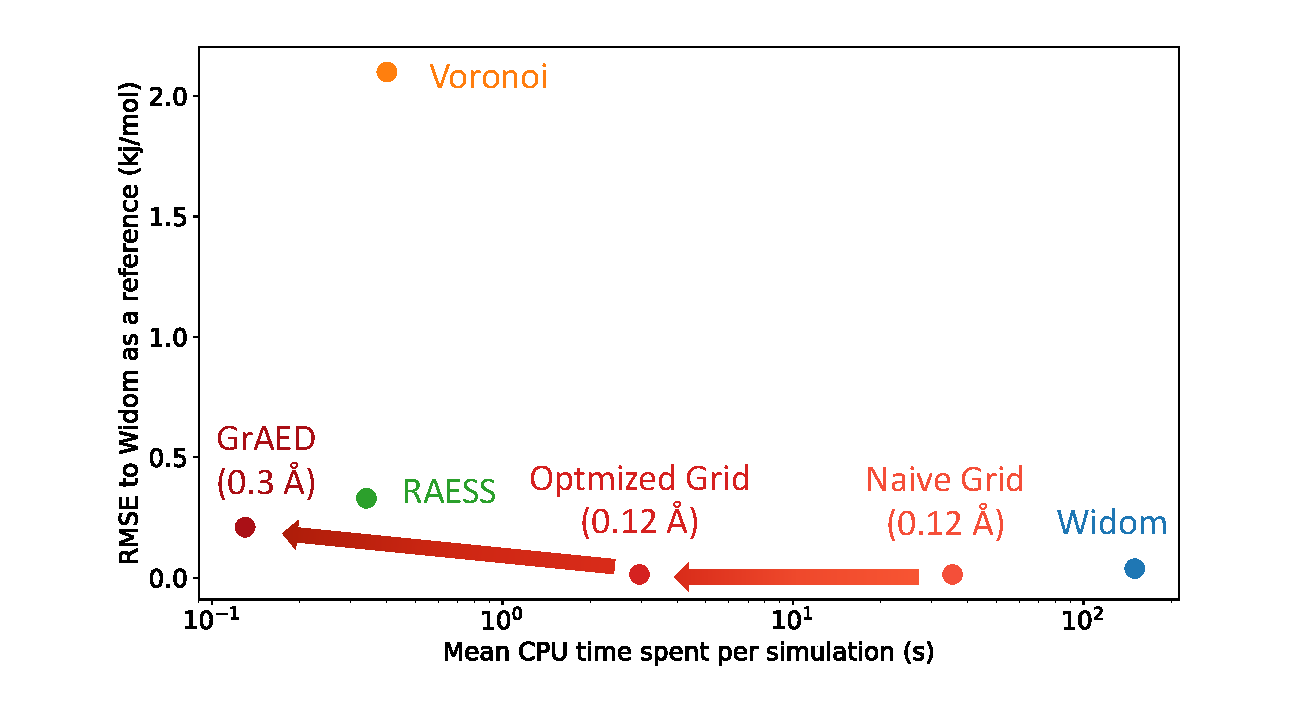
\includegraphics[width=0.7\textwidth]{figures/3-fastsim/Grid_sumup.pdf}
      \caption{Comparaison de la racine de l'erreur quadratique moyenne sur l'enthalpie d'adsorption du xénon et le temps de simulation par structure pour différentes méthodes d'échantillonnage  sur la base de données CoRE MOF 2019 (pour une taille de pore supérieur à \SI{3.7}{\angstrom}). }\label{fgr:grid_perfomance}
  \end{figure}

\todo{ML}

\section*{Propriétés de transport}

\begin{figure}[ht]
    \centering
      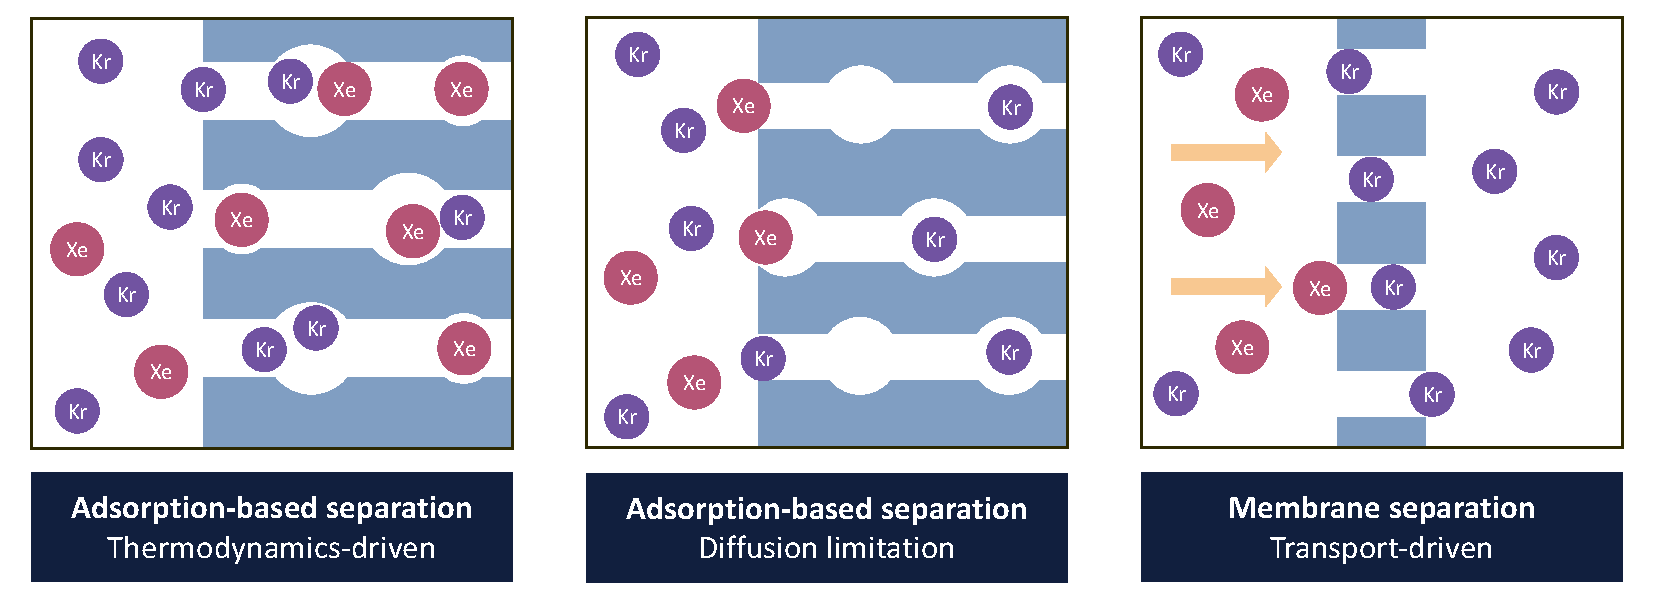
\includegraphics[width=0.95\textwidth]{figures/5-diffusion/Diffusion.pdf}
      \caption{Illustration of the comparative role of the thermodynamic and transport properties for Xe/Kr separation in nanoporous materials. From the transport dominated process of membrane separation to the thermodynamically equilibrated separation processes in the nanopores, different more nuanced cases could emerge where the diffusion imposes kinetic limitations.}\label{fgr:intro_diffusion}
  \end{figure}

\todo{correlation}

\begin{figure}[ht]
\centering
\begin{subfigure}[b]{0.48\textwidth}
    \centering
    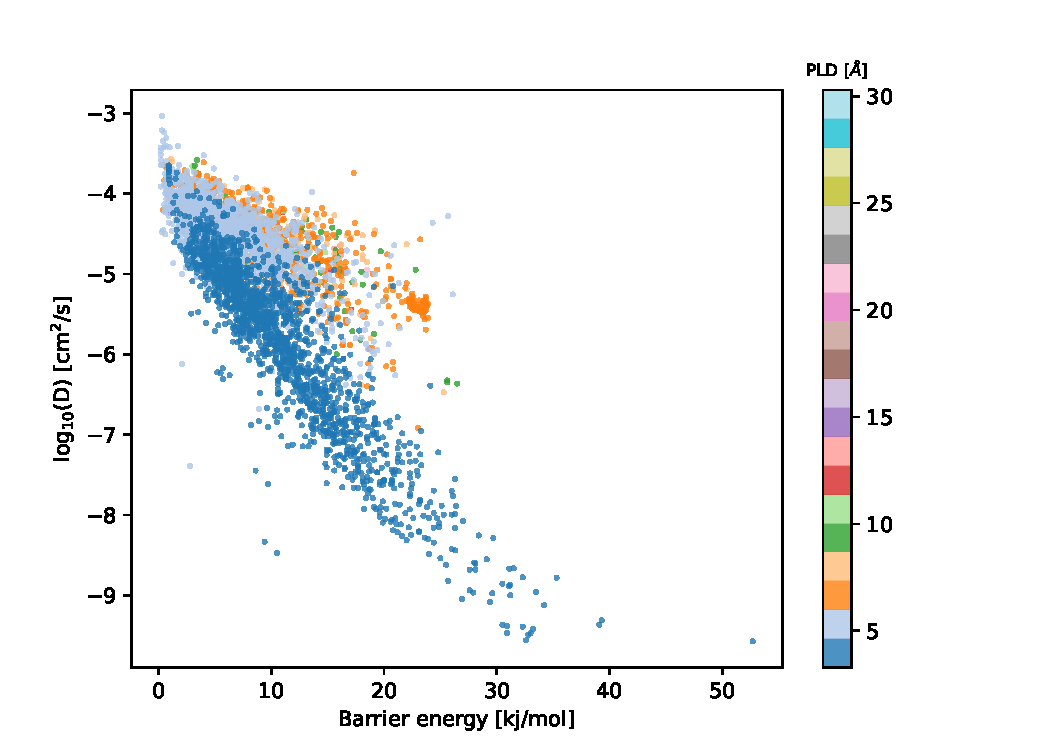
\includegraphics[width=\textwidth]{figures/5-diffusion/difflog_barrier_Df_uff.pdf}
    \caption{Energy barrier}\label{fgr:barrier_diffusion_a}
\end{subfigure}
\hfill
\begin{subfigure}[b]{0.48\textwidth}
    \centering
    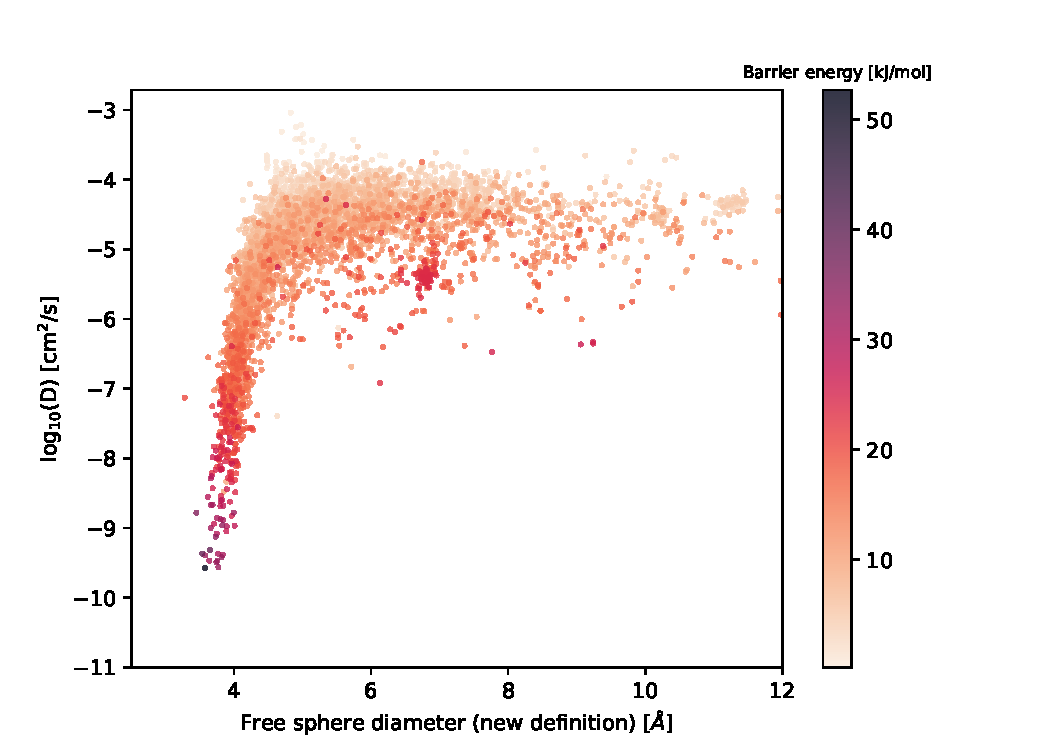
\includegraphics[width=0.6\textwidth]{figures/5-diffusion/difflog_Df-uff298K_barrier.pdf}
    \caption{PLD}\label{fgr:barrier_diffusion_b}
\end{subfigure}
    \caption{ Scatterplots of the $\log_{10}$ of the diffusion coefficient (in \si{\square\cm\per\s}) compared to the barrier activation energy $E\e{a}$ in \si{\kJ\per\mol} (a) for all structures  and (b) for the structures with a PLD over \SI{6}{\angstrom}.}\label{fgr:barrier_diffusion}
\end{figure}

\todo{ML}

\begin{figure}[ht]
\centering
    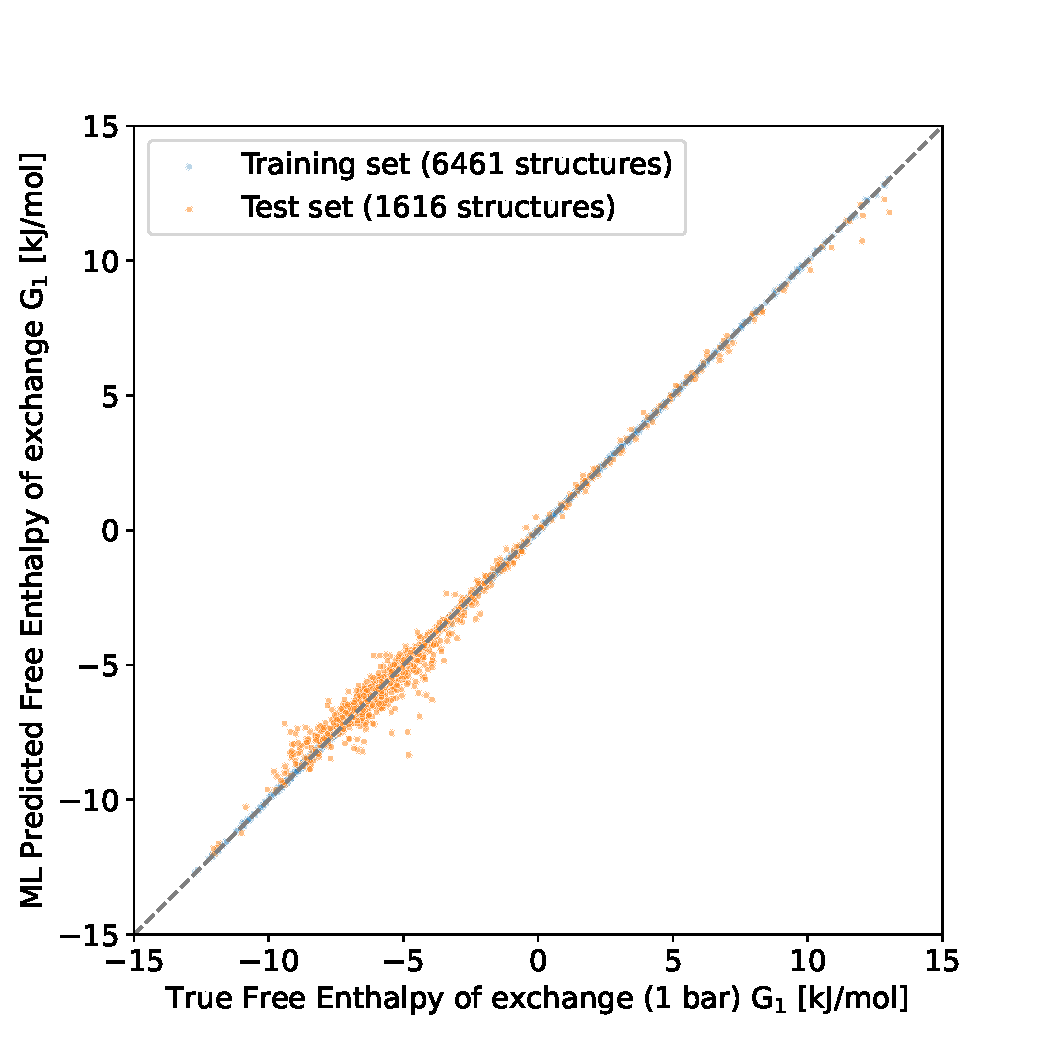
\includegraphics[width=0.5\linewidth]{figures/4-ml/main/Scatterplot_G1_prediction.pdf}
    \caption{Scatter plot of the exchange free energy predicted by the model. There is a good agreement between the predicted and true values. On the test set, there is an RMSE of \SI{0.37}{\kilo\joule\per\mole} and an MAE of \SI{0.21}{\kilo\joule\per\mole}. This plot is equivalent to the scatter plot between the logarithm of the ambient-pressure selectivity (see Figure~\ref{fgr:S1_prediction}). The corresponding errors for the ambient-pressure selectivity are 2.5 and 1.1 for respectively the RMSE and MAE of the selectivity, and 0.065 and 0.038 for the RMSE and MAE of its base-10 logarithm. }\label{fgr:G1_prediction}
\end{figure}

\begin{figure}[ht]
    \centering
        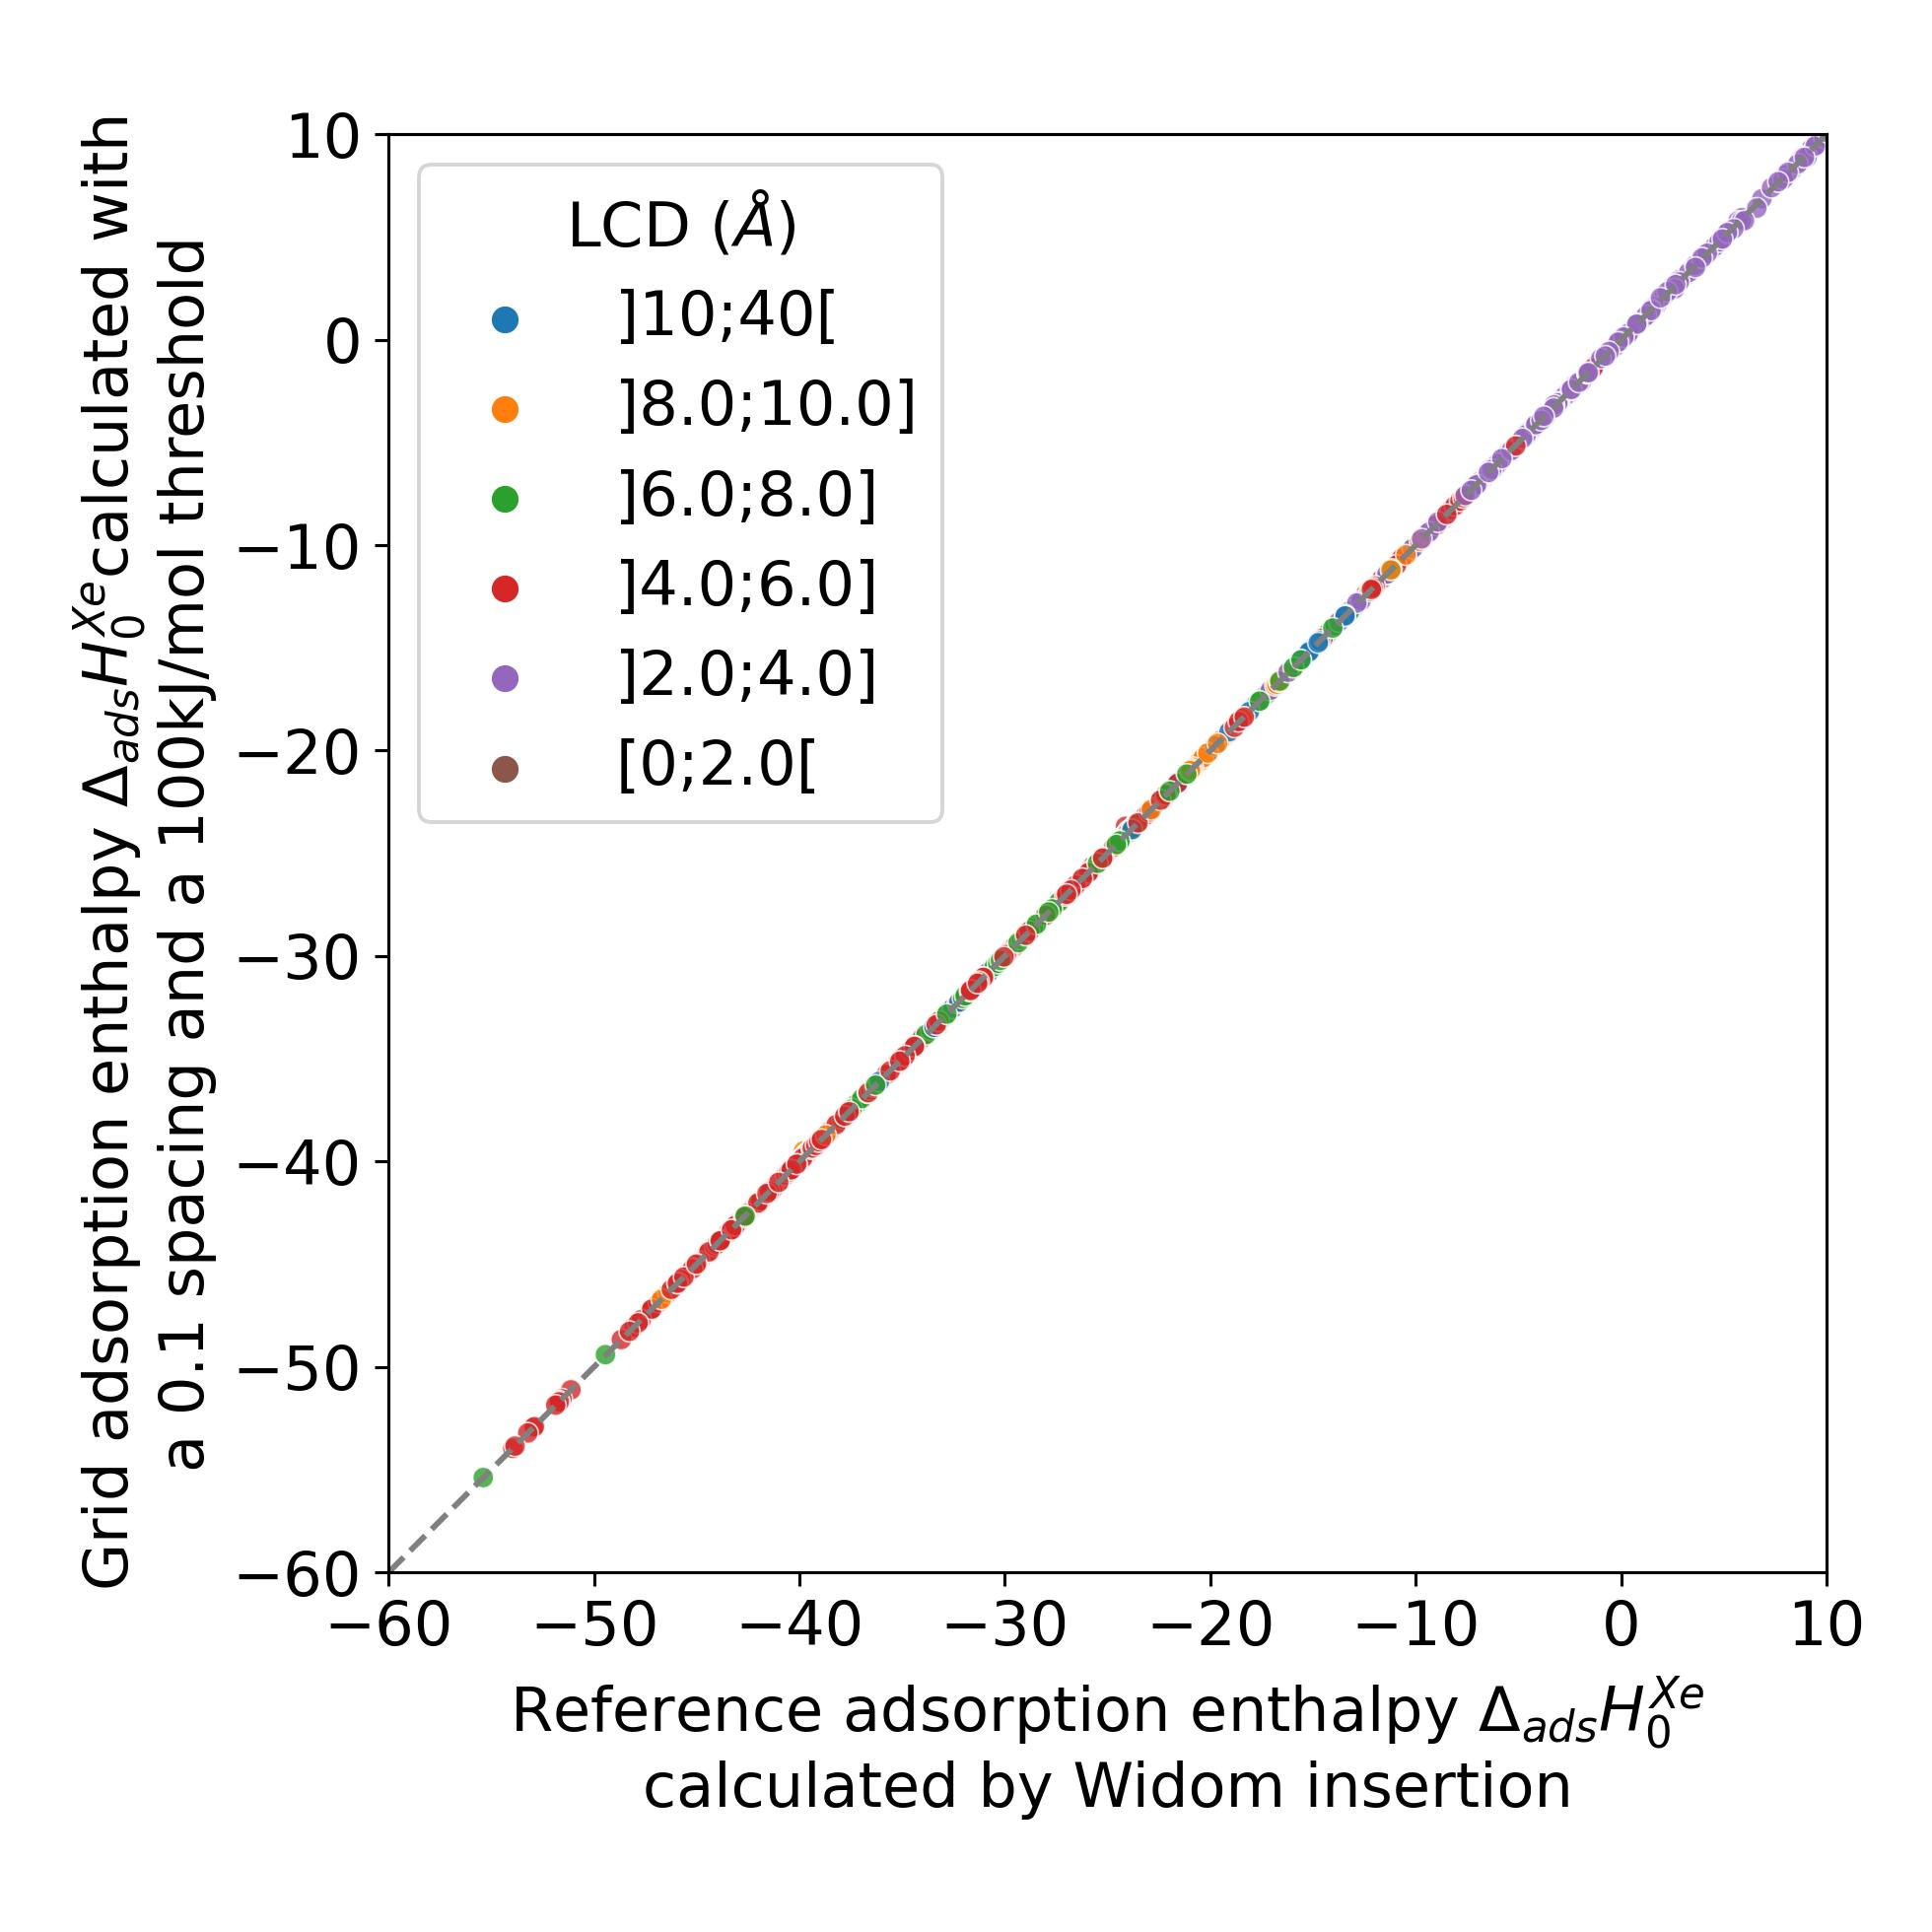
\includegraphics[width=0.45\textwidth]{figures/3-fastsim/H_Xe_widom_vs_H_Xe_grid_overview.jpg}
        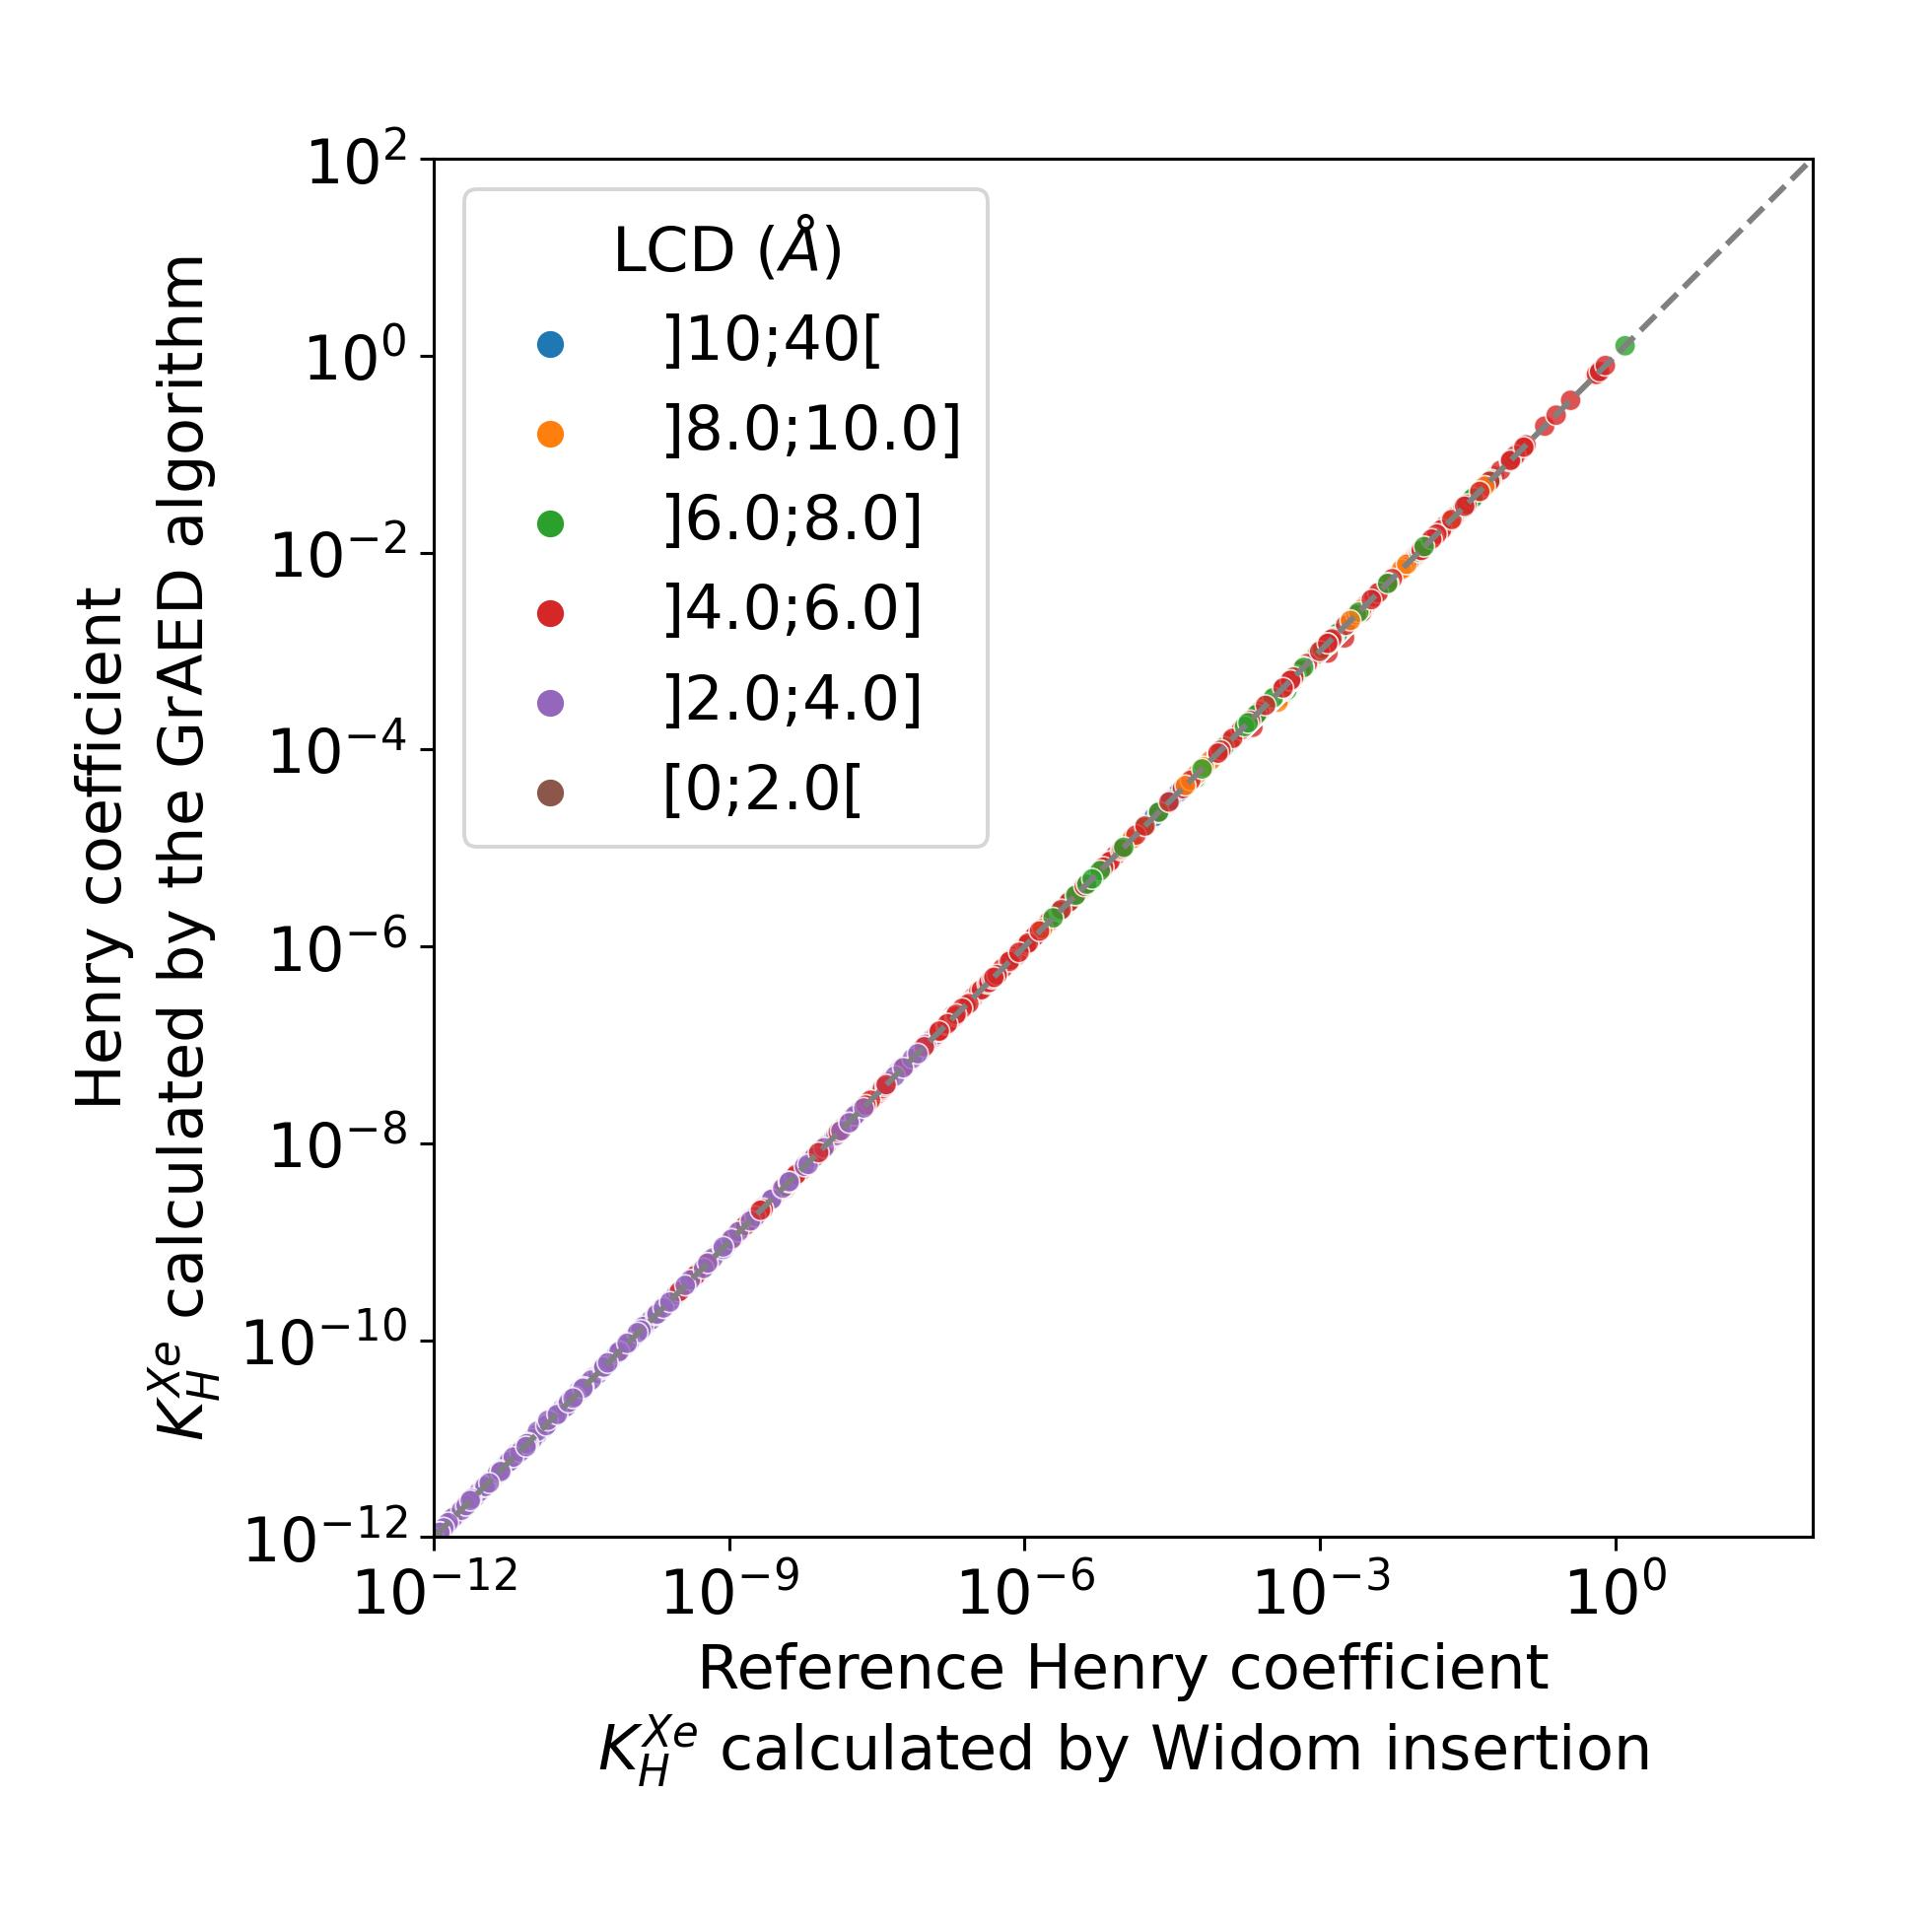
\includegraphics[width=0.45\textwidth]{figures/3-fastsim/K_Xe_widom_vs_K_Xe_grid_overview.jpg}
        \caption{Comparison of the xenon adsorption enthalpies (left) and the Henry constants (right) calculated by the optimized grid energy sampling (for a \SI{0.12}{\angstrom} spacing, a rejection parameter $\mu=0.8$ and an energy threshold $E\e{th}$ of \SI{100}{\kilo\joule\per\mole}) and by the Widom insertion of RASPA2 with 100,000 cycles on the CoRE MOF 2019 structures (LCD\e{CCDC} $\geq$ \SI{3.7}{\angstrom}). }\label{fgr:grid_widom}
    \end{figure}

\section*{Conclusion}

\begin{figure}[ht]
    \centering
    \begin{subfigure}[b]{0.48\textwidth}
      \centering
      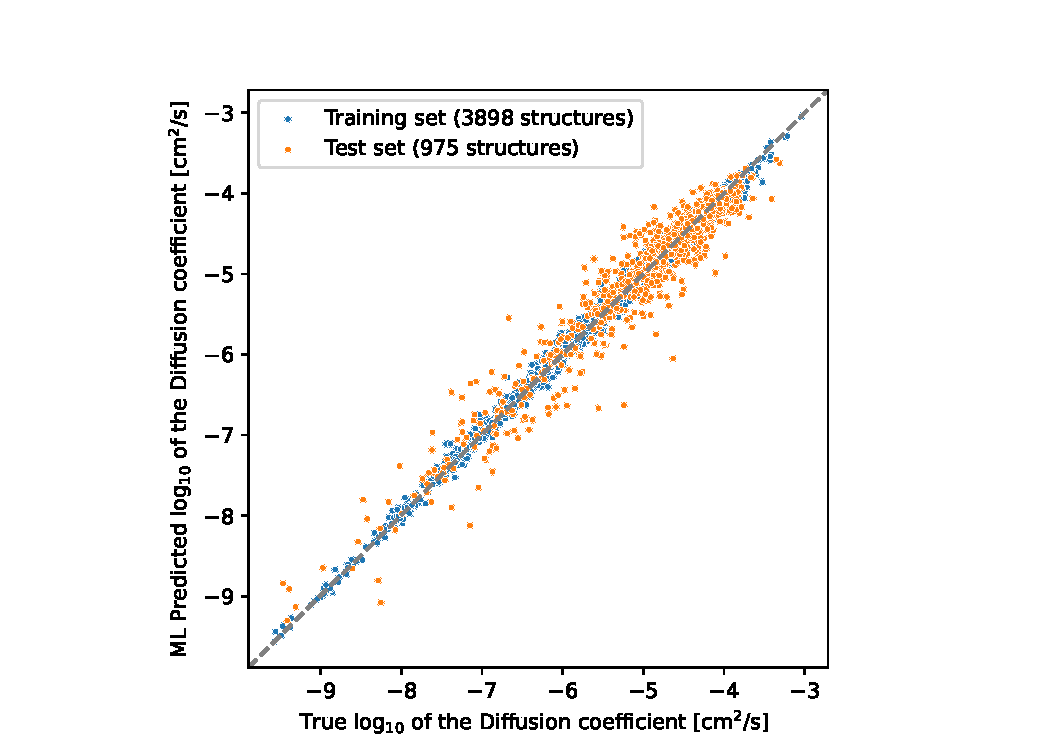
\includegraphics[width=\textwidth]{figures/5-diffusion/diffusion_prediction.pdf}
    \caption{Prediction result}\label{fgr:diffusion_pred}
    \end{subfigure}
    \begin{subfigure}[b]{0.48\textwidth}
      \centering
      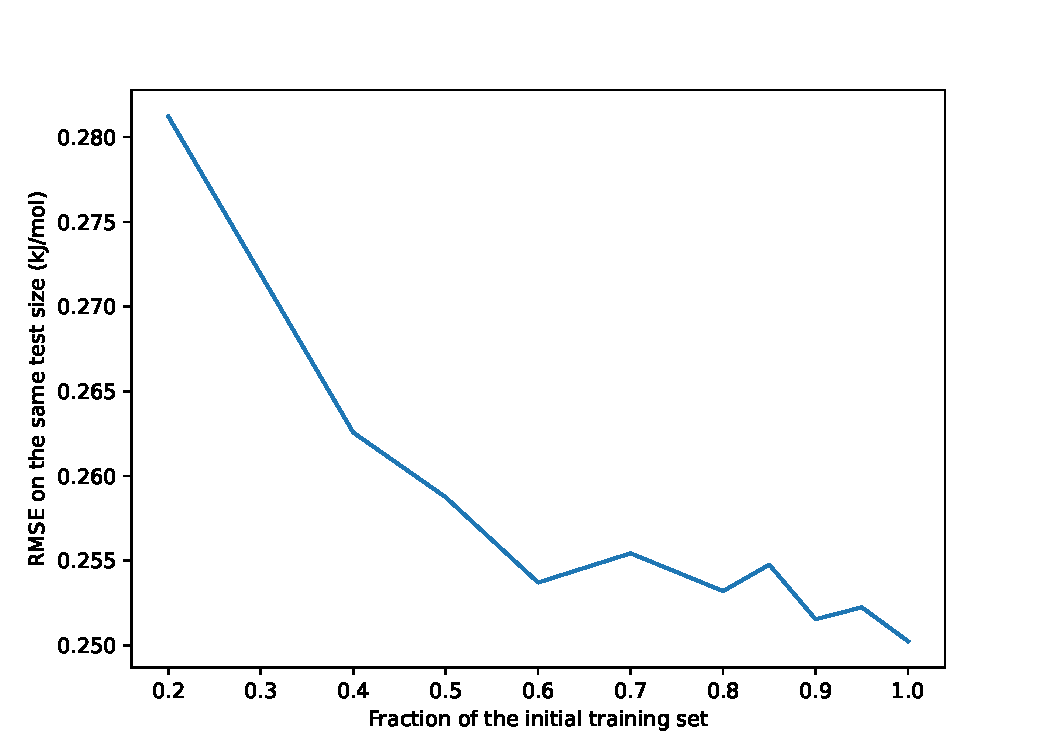
\includegraphics[width=\textwidth]{figures/5-diffusion/training_curve.pdf}
      \caption{Training curve}\label{fgr:training_curve_diff}
    \end{subfigure}
      \caption{ (a) Comparison of the $\log_{10}$ of the diffusion coefficient predicted by an ML model and the true values. (b) Root mean squared errors on the same test set (20\% of all data) as a function of the fraction of the training set used to train smaller models. The error decreases as the amount of data increases and seems to stabilize near $0.25$. }
  \end{figure}

\vfill
\begin{center}
    \pgfornament[width=6cm,color=CTsemi]{75}
\end{center}
\vfill\vfill

\end{otherlanguage}

\OnlyInSubfile{\printglobalbibliography}

\end{document}
